\documentclass{standalone}
\usepackage{tikz}
\usetikzlibrary{positioning}
\begin{document}
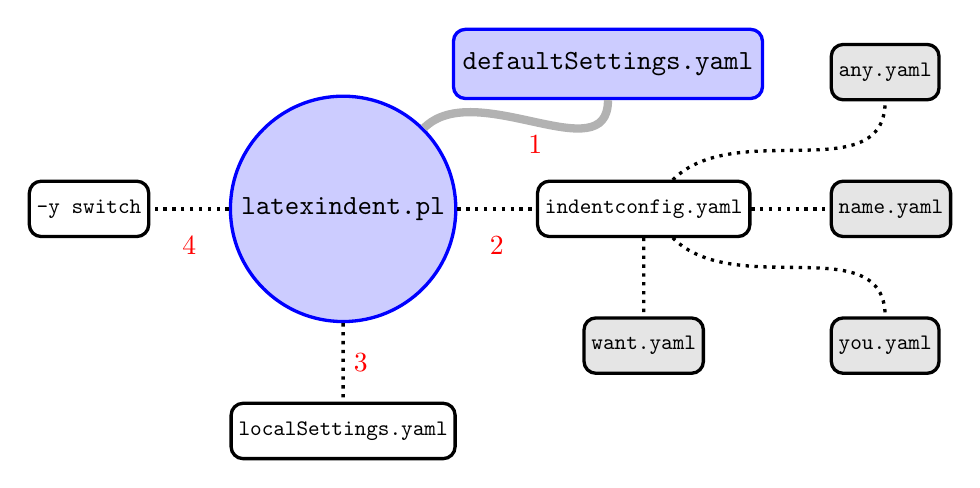
\begin{tikzpicture}[
		needed/.style={very thick, draw=blue,fill=blue!20, text centered, minimum height=2.5em,rounded corners=1ex},
		optional/.style={draw=black, very thick,scale=0.8, text centered, minimum height=2.5em,rounded corners=1ex},
		optionalfill/.style={fill=black!10},
		connections/.style={draw=black!30,dotted,line width=3pt,text=red},
	]
	% Draw diagram elements
	\node (latexindent) [needed,circle] {\texttt{latexindent.pl}};
	\node (default) [needed,above right=.5cm of latexindent] {\texttt{defaultSettings.yaml}};
	\node (indentconfig) [optional,right=of latexindent] {\texttt{indentconfig.yaml}};
	\node (any) [optional,optionalfill,above right=of indentconfig] {\texttt{any.yaml}};
	\node (name) [optional,optionalfill,right=of indentconfig] {\texttt{name.yaml}};
	\node (you) [optional,optionalfill,below right=of indentconfig] {\texttt{you.yaml}};
	\node (want) [optional,optionalfill,below=of indentconfig] {\texttt{want.yaml}};
	\node (local) [optional,below=of latexindent] {\texttt{localSettings.yaml}};
	\node (yamlswitch) [optional,left=of latexindent] {\texttt{-y switch}};
	% Draw arrows between elements
	\draw[connections,solid] (latexindent) to[in=-90]node[pos=0.5,anchor=north]{1} (default.south) ;
	\draw[connections,optional] (latexindent) -- node[pos=0.5,anchor=north]{2} (indentconfig) ;
	\draw[connections,optional] (indentconfig) to[in=-90] (any.south) ;
	\draw[connections,optional] (indentconfig) -- (name) ;
	\draw[connections,optional] (indentconfig) to[out=-45,in=90] (you) ;
	\draw[connections,optional] (indentconfig) -- (want) ;
	\draw[connections,optional] (latexindent) -- node[pos=0.5,anchor=west]{3} (local) ;
	\draw[connections,optional] (latexindent) -- node[pos=0.5,anchor=north]{4} (yamlswitch) ;
\end{tikzpicture}
\end{document}
